\title{PLUTO simulation and imaging procedures}
\author{Jonathan Rogers}
\date{\today}
\documentclass[12pt]{article}

\usepackage{graphicx}
\usepackage{amsmath}
\usepackage{verbatim}

\usepackage{listings}
\usepackage{color}

\definecolor{dkgreen}{rgb}{0,0.6,0}
\definecolor{gray}{rgb}{0.5,0.5,0.5}
\definecolor{mauve}{rgb}{0.58,0,0.82}

\lstset{frame=tb,
	language=Python,
	aboveskip=3mm,
	belowskip=3mm,
	showstringspaces=false,
	columns=flexible,
	basicstyle={\small\ttfamily},
	numbers=none,
	numberstyle=\tiny\color{gray},
	keywordstyle=\color{blue},
	commentstyle=\color{dkgreen},
	stringstyle=\color{mauve},
	breaklines=true,
	breakatwhitespace=true,
	tabsize=3
}

\begin{document}
\maketitle

\noindent This document outlines the general processes required to simulate, in 2D, an astrophysical jet using PLUTO. It also provides general instructions on imaging your simulation using python. \\
\newline
Note that it is assumed that the user has python 2.7 installed, as the pyPLUTO python module that comes with PLUTO does not work in python 3.
\section{PLUTO}

PLUTO is a user-friendly finite-volume (finite-area in 2D case), shock-capturing code that was written (in C) to integrate a set of conservation laws such as the hydrodynamical equations. There are four inbuilt physics modules allowing for hydrodynamical, magnetohydrodynamical, special relativistic hydrodynamical, and relativistic magnetohydrodynamical physics to be investigated.\\
\\
After initial installation (which is beyond the scope of this document), the code requires 4 files to run: init.c, definitions.h, pluto.ini and an appropriate makefile for your OS. The following sections summarise the role of each of these files, and give a brief how-to on setting up your own simulation with an emphasis on producing astrophysical jets. The latter sections discuss imaging your simulation using python. A more in-depth guide to PLTUO can be found in the userguide at http://plutocode.ph.unito.it/files/userguide.pdf.

`The idea is that a new user with a fresh install can start here, but those wishing to understand how to completely customise your simulation will need to refer to the userguide' 
\subsection{Simulation set up}

The three important files that govern the behaviour of your simulation are the definitions.h, pluto.ini and init.c files. These files define things such as the physics, resolution, values of your input parameters (eg, Mach numbers, densities and pressures), temporal parameters such as how often results are printed to file, or the simulation length, and the time dependent boundary conditions. The files are not independent of each other - that is, there are options that are 'switched on' in one file, but given a value in another.

\subsubsection{definitions.h}
The definitions.h file specifies which fluid equations will be solved, how they will be solved (Rieman solver and time stepper) and what user defined parameters exist. There are also some other physics dependent parameters such as which equation of state should be used, and whether the equation of entropy should be added to the conservation laws, but these will not be discussed.\\
\\
It is also important to note that the definitions.h file can be configured by running the setup.py script (located in the PLUTO/ folder by default). However, there are some parameters that must be edited manually.

\paragraph{Physics and geometry}\mbox{}
\newline
Selecting a physics module - and thus determining which fluid equations will be solved - is done so by setting the `PHYSICS' parameter. As the aim of this document is to enable the reader to run a simple hydrodynamic simulation (negating magnetic fields or relativistic effects), the PHYSICS parameter should be set to HD. The HD option will assume classical hydrodynamics as described by the Euler equations (see section 6.1 of the userguide for more information).

The geometry, number of dimensions and the number of vector components are set via their corresponding parameters.

DIMENSIONS              2
COMPONENTS              2
GEOMETRY                SPHERICAL (eg, (x1,x2) = (r,$\theta$)
BODY\_FORCE              POTENTIAL (can also be VECTOR)

\paragraph{Solvers}
keywords: RECONSTRUCTION, TIME\_STEPPING
These 2 are important, but see Martins lectures on the utas-AGN github (or dropbox?) for a better discussion
RECONSTRUCTION          LINEAR
TIME\_STEPPING           RK2


\paragraph{Defining parameters}
Keywords: NTRACER, USER\_DEF\_PARAMETERS, EOS
NTRACER                 1
USER\_DEF\_PARAMETERS     2

In the pysics dependent declarations for simplicity we will assume that the gas behaves as an ideal gas. This is done by setting the equation of state (EOS) to IDEAL.
\#define  EOS                     IDEAL

The user defined paramaters section is where you define new variables in the simulation. the number of variables here must match the number of USER\_DEF\_PARAMETERS set in the first section of the file.
\#define  H\_OPEN\_ANG              0
\#define  MACH\_EXT                1


\#define  PRINT\_TO\_FILE       YES
outputs the log to pluto.log, extremely useful for troubleshooting

- number of user defined parameters in the third block must match the value of USER$\_$DEF$\_$PARAMETERS in the first block.

- the geometry and body force selection must match the coding of your simulation in the init.c file

- max number of tracers accepted when running setup.py is 8, any more and you will need to manually edit the definitions.h file. Also any more than 8 and you won't be able to look at all of the parameters using the GUI as it is not optimized more >8 tracers.
\paragraph{Importance of geometry in jet simulations}\mbox{}
\newline
- can specify opening angle of jet in terms of theta (mention Krause et al. 2012 and how it is a morpholoy divide between jets)

\subsubsection{pluto.ini}
“pluto.ini (sets the number of grid zones, Riemann solver, output frequency, etc.),”
Selecting your grid
spherical coordinates\\
\\
The [Grid] section enables for resolution customisation of the simulation grid space. This is useful as finer grid spacings are required in some important areas of jet simulations. For example, in areas around the jet-environment boundary, a higher resolution grid is needed to be able to resolve turbulence. This is vitally important as turbulence plays a large role in momentum transfer from jets, causing differing morphologies (e.g. Perucho DATE). \\
the simulation grid is composed of 'grid patches'. Each grid patch may differ in:- 
\begin{itemize}
\item Size
\item Number of cells
\item Size of the cells comprising the patch; or
\item How the cells are distributed over the patch
\end{itemize}
For example, figure 1 below shows a 2D grid space extending out to x = 12.  There are 2 patches (as indicated by the shading). Patch 1 is 0 $\leq x < 6$ and contains 6 cells in x. Patch 2 is 6 $\leq x <$ 12 and contains half the amount of cells 3 cells. This is useful if finer resolution is needed for 'what is going on' below x = 6, and not required at lengths larger than that, and therefore the computation time benefits from the smaller grid.


The y direction is uniform - meaning that there is only 1 patch in the y direction.


The spacing of the cells in the $\hat{y}$ direction is larger for 5 < x <= 9
\begin{figure}[h]
	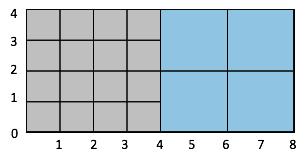
\includegraphics[width=8cm]{gridspaces}
	\centering
	\caption{Grid with even spacing in $\hat{y}$, but two patches with different spacings in $\hat{x}$}
\end{figure}


Write about tmax and dt
Write about output frequency
\subsubsection{init.c}
Setting up an environment
boundary condition\\
\\
the init.c file sets up the boundary conditions (which are a function of time) of your simulation grid. The manipulation of the lower (x,y) boundary (or lower (r) boundary on a spherical grid) to include an inflow of conserved simulation quantities is used to simulate a fluid jet. These quantities can also be user defined (see definitions.h section).

need to put in the actual code here and talk about it. show code for
'initial conditions'
'user defined boundary conditions'
'gravity bit at the end'

\subsection{Nondimensionalization of the simulation}
- Two limitations of numerical simulations are computation time, and numerical errors. 
- Both of these factors can be optimized by either increasing the amount of memory avaliable, or reducing the amount of memory that your code uses.
- Both computing large numbers (in absolute value), and storing these values in memory is expensive.
- These issues can be addressed through the normalisation of your simulation parameters.
- Handy to normalise the values to one of the length scales outlined in Krause et al. 2012

\subsubsection{Characteristic length scales of astrophysical jets}
- There are two bounding length scales, L1 and L2.
- L1 is where ...
- L2 is where ...
- There are three other applicable length scales that can exist between these - L1a, L1b, and L1c. Named in sequential order as they usually exist in that manner

There are two bounding length scales to consider (as derived by Alexander?) referred to as L1 and L2. L1 is the distance from the AGN that the jet density approaches the environment density, i.e.
\begin{equation}
\text{L1: }\rho_{jet} = \rho_x
\end{equation}
This is typically referred to as the inner scale. why?\\
The outer scale of a jet, or L2 is where the jet pressure is comparable to the environment pressure, i.e.
\begin{equation}
\text{L2: }P_{jet} = P_{x}
\end{equation}
Note that the environment pressure and density could refer to the ambient medium, or the jet cocoon should one have formed.\\
\\
There exist three more length scales between L1 and L2. However, unlike the inner and outer scale, the order of the remaining three scales depend on the physics of the jet and environment, and will determine the morphological features of the jet and the surrounding medium.

The remaining three length scales relate to the locations of jet collimation (L1a), cocoon formation (L1b) and jet termination (L1c). Note that there is no order to these three scales, and thus jet morphology can be understood via the ratios of the scales. It is important to note that the scales discussed at not locations where these processes happen, but rather order of magnitude estimates.\\
\\
L1a: Scale of jet collimation.\\
Collimation happens on scales where the sideways ram pressure of the jet starts to fall below the environmental pressure. I.e.
\begin{equation}
\rho_{jet}v_{jet}^{2}\sin{\theta} < P_{x}
\end{equation}
Where subscript \textit{x} refers to the environment immediately outside the jet, and $\theta$ is the half opening angle of the jet.\\
\\
L1b: Scale of cocoon formation
The scale on which the jet density falls below the density of the environment. Should a cocoon form before the jet collimates (i.e. L1a/L1b < 1), then for the purposes of L1a, the subscript x refers to the cocoon.\\
\\
L1c: Scale of jet termination
A jet termination shock appears on scales of L1c. At L1c, the forward ram pressure of the jet falls below the environmental density. Should the scale of L1b be smaller than L1c, then this environment refers to the cocoon.\\
\\
Krause et al. 2012 discusses the derivation of these length scales in some detail, calling on work from Komissarov \& Falle 1998, and Alexander 2006. However, the length scales calculated relate to an environment of constant density. Hardcastle \& Krause 2013 used these length scales in numerical modelling of radio galaxy globes in cluster (non-constant) environments.

note about the text doc that i wrote to myself in the dropbox. HK13 uses a unit density to calculate L2, where $\rho_0 = n_0\mu m_p$. So it doesn't matter that it's a function of radius. I need to choose an approprate value of $n_0$. HK13 uses 3$\times$10$^4$m$^{-3}$.

FIX UP THE ABOVE, PROBABLY NEEDS TO BE REWRITTEN A LITTLE BIT, AND MAYBE PUT IN A PIC FROM KRAUSE2012 SHOWING THAT THE JET COLLIMATES ON A SCALE OF 1 WHICH IS HIS NORMALISATION SCALE I THINK (I.E. L1A).\\
\\
Need to rewrite equations in terms of jet power, density and velocity. i.e. just the equations that are in the 2012 paper (remember to correct them).

\begin{comment}
pythoncode:
Calculate Q0, rho, Mach number (vj/cs) 

def CalcL1(Q0, rho, vjet):
L1 = 2.0*np.sqrt(2.0)*np.sqrt(Q0/(rho*vjet**3)).to(u.parsec)
return L1

def CalcL2(Q0,rho,cs):
L2 = np.sqrt(Q0/(rho*cs**3)).to(u.kiloparsec)
return L2

def timeUnit(L1,cs):
tau = (L1.to(u.m)/cs.to(u.m/u.second)).to(u.year)
return tau
\end{comment}

need to add that you need to run make, and then what will get output.
\subsection{Viewing your data}
There is an pre-coded GUI that uses the pyPLUTO python module to display 2D images, or slices of your simulation output. However, the resolution at which the GUI displays the data is less than the actual resolution of the simulation (this is usually the case when the grid spacing is low enough to resolve turbulence). It is easier to get a better quality image by importing the pyPLUTO module into pluto yourself, and manually extracting, then imaging the data yourself. This section outlines how to use the pyPLUTO code, how to create images, and a small introduction to making movies of your simulations.

\subsubsection{pyPLUTO module}
pyPLUTO is a pluto module developed by Bhargav Vaidya and Denis Stepanovs, and is extremely useful for analysing PLUTO simulations. Within the module is the function pload, which creates a pyPLUTO object with attributes that include the output matrices of your simulation, grid information and information on the simulated quantities. The function requires two inputs:
\begin{itemize}
\item ns: the output file number (eg, 0 would be the output binary file data.0000.dbl)
\item run\_dir: the directory that your simulation resides in
\end{itemize}
For example, to load the density map of your simulation:
\begin{lstlisting}
import pyPLUTO as pp

ns = 1 #define output file to analyse
run_dir = 'MyDirectory/MyPlutoSimulation/' #set run directory
curObject = pp.pload(ns,run_dir) #create pyPLUTO object
density = curObject.rho #get attribute (density in this case) from the pyPLUTO object
X1_AXIS = curObject.x1 #get x axis of simulation, is a vector
X2_AXIS = curObject.x2 #get y axis of simulation, is a vector
\end{lstlisting}
It is often useful to define simulations of astrophysical jets in spherical coordinates (see section x), in which case the X1\_vector and X2\_vector would actually represent the (R,$\Theta$) axes.\\
is there ay more to say?

\subsubsection{Plotting with matplotlib}

Set up a grid using meshgrid
\begin{lstlisting}
import numpy as np
import matplotlib.pyplot as plt

#Create a grid by producing a 2D array of the combination of the values in the two *_AXIS vectors
X1, X2 = np.meshgrid(X1_AXIS, X2_AXIS)

#Create the density map using the pcolormesh plotting function 
plt.pcolormesh(X1,X2,density)

#Set axis lavels
plt.xlabel('x')
plt.ylabel'y')

#Add a colorbar
cb = plt.colorbar()

#Display the plot
plt.show()
\end{lstlisting}

\begin{figure}[!h]
	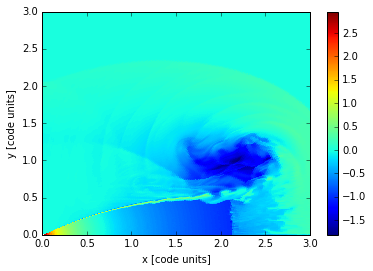
\includegraphics[width=15cm]{examplesim}
	\centering
	\caption{caption}
\end{figure}


Alternatively, is it better practise to write functions for getting the data and plotting it
Making a movie

\section{PLUTO Example}
Require the user to download some example files from gitgub
- probably also talk about how to put your own files on github, giving special care not to prompt the user to upload their entire simulation.


\subsection{}

TO DO ON MY AUSCOPE SHIFT :D (hopefully..)
- copy jet example
- download the init.c, definitions.h and pluto.ini file from github
- configure it to be in spherical coordinates
- plot in R,Theta space
- transform to cartesian and replot
\end{document}